\documentclass[a4paper]{article}

% Packages
\usepackage{geometry}
\geometry{left=1.5cm, right=1.5cm, top=2.54cm, bottom=2.54cm}
\usepackage{graphicx, hyperref, setspace, amsmath, amssymb, titlesec, multicol, parskip, indentfirst, etoolbox, caption, xcolor, svg}
\usepackage[style=ieee]{biblatex}
% Import the bibliography file
\addbibresource{ref.bib}

% Title Formatting
\titleformat{\section}{\centering\large\scshape}{\thesection}{1em}{}
\titleformat{\subsection}{\normalsize\bfseries}{\thesubsection.}{1em}{}
\setstretch{1.0} % Keep single spacing
\setlength{\parskip}{6pt} % Space between paragraphs
\titlespacing{\section}{0pt}{6pt}{6pt}
\titlespacing{\subsection}{0pt}{6pt}{6pt}
\titlespacing{\subsubsection}{0pt}{6pt}{6pt}
% Document Title
\title{
    \textbf{Draft v2}
}

\date{}
\captionsetup{labelfont={small,sc}, textfont={small,sc}, hypcap=false}
%\captionsetup{labelfont={small,sc}, textfont={small,sc}}
% Section Numbering
% Define numbering format
\renewcommand{\thesection}{\Roman{section}.}
\renewcommand{\thesubsection}{\textit{\Alph{subsection}.}}
\renewcommand{\thesubsubsection}{\textit{\arabic{subsubsection}.}}
\renewcommand{\thetable}{\Roman{table}} % Set table numbering to Roman
\renewcommand{\thefigure}{\Roman{figure}} % Number figures in Roman numerals

% Make subsection titles italic as well
\titleformat{\subsection}{\normalfont\large\itshape}{\thesubsection}{1em}{}
\titleformat{\subsubsection}{\normalfont\itshape}{\thesubsubsection}{1em}{}

\begin{document}

\maketitle
\vspace{-1.5cm}

% Authors Block
\begin{multicols}{3}
    \centering
    \textbf{Yang Li}\\
    \textit{University of the West of England}\\
    \textit{yang4.li@uwe.ac.uk}\\
    \vfill

    \textbf{Marco Perez Hernandez}\\
    \textit{University of the West of England}\\
    \textit{marco.perezhernandez@uwe.ac.uk}\\
    \vfill

    \textbf{Mehmet Aydin}\\
    \textit{University of the West of England}\\
    \textit{mehmet.aydin@uwe.ac.uk}\\
    \vfill
\end{multicols}

\singlespacing
\setlength{\parskip}{6pt}
\setlength{\parindent}{0.5cm}

\begin{abstract}
The abstract should be written after the rest of the paper is completed.
\end{abstract}

\begin{multicols}{2}
\setlength{\columnsep}{0.5cm}

\section{Introduction}
Many real-world problems can be modelled as non-cooperative games, such as business competition, political campaigns, stock trading, bidding in auctions, cyber security, and traffic routing. These problems feature the competitive nature of games because they share one thing in common, parties with conflicting interests. Plenty of research has been done on multi-agent reinforcement learning (MARL) in fully cooperative games. There is currently a gap in the non-cooperative setting \cite{zhu2024survey}. Most current SOTA MARL algorithms are designed for cooperative games.

In fully cooperative games, there is no conflict between agents. If agents can communicate, they are motivated to form a firm alliance that essentially works as a collective mind that is the one and only conscious being. Thus, in a game theory sense, a fully cooperative game where agents share information is equivalent to a single agent game where the collective agent tries to find the optimal joint action, given the joint observation. To do that in a traditional single agent setting where the environment is stationary and non-adversarial, one only needs to learn the environment mechanics (the state transition function) and the reward function so that the Q-values of an action in a given state can be computed or predicted by a function approximator. A Pareto optimal pure (deterministic) strategy is guaranteed to exist in fully cooperative finite games, meaning that the agents can always deterministically choose the optimal action that has the highest payoff. The only thing that keeps the agents from forming a cluster in practice is the hardware incapability (computational power, real-world constraints, etc.).

Non-cooperative environments, however, involve conflicts that make learning more complicated. Agents may belong to different parties that would like to have private control to protect their own interests. For example, the stock market is often considered a 0-sum fully competitive game where one person's profit is another person's loss, if we omit the long-term economic growth, especially when we consider options, futures, etc. Another example is cyber security, which must study the conflicts between attackers and defenders.

For cooperative games, we can always say that 5 rewards is better than 2 rewards, but what about the rewards $\langle 1,5 \rangle$ and  $\langle 10,1 \rangle$ where each agent gets one value in the vector? Rational self-interested agents will have to fight for what is best for them. Many solutions in game theory are possible. One of the commonly accepted solutions is the Nash equilibrium (NE). NE describes a situation where no player can benefit by deviating from their current strategy independently. NEs are normally what we want the agents to converge to because convergence means stability and strict NEs are the only stable points in the game. Generally, there may only be a mixed NE, meaning that players adopt randomized strategies consisting of probability distributions over the action space.

Currently, most SOTA MARL algorithms cannot learn a mixed policy. Largely due to the studied games are mostly fully cooperative or asynchronous. As we will show in the experiments, those algorithms will fail to find the optimal action in games specifically designed to challenge the agents' competitive thinking. We need to reconsider our approach if we want to build agents that are capable of dealing with non-fully-cooperative environments.

\subsection{Aim}
The aim of this study is to point out that current SOTA algorithms can be misleadingly performing well in non-fully-cooperative environments. Furthermore, we will find out the conditions a game must satisfy for the algorithms to work by both formal analysis and specific game scenarios that are designed to challenge the agents from a game theory perspective.

\subsection{Stochastic Game}

A (finite) stochastic game is formally defined by a tuple:

$G = \langle I,S,S_0,S_t,\{A_1,\ldots,A_n\},\{R_1,\ldots,R_n\},T \rangle$
\begin{itemize}
    \item $I$: the set of agents, numbered from 1 to $n$.
    \item $S$: the game’s state space.
    \item $S_0$: the set of possible initial states.
    \item $S_t$: the set of terminal states.
    \item $\{A_1,\ldots,A_n\}$: one action space for each agent.

    Let $a_i \in A_i$ be an action of agent $i$, and $a^n=\langle a_1,\ldots,a_n \rangle \in A^n$ denote a joint action in the joint action space.
    \item $\{R_1,\ldots,R_n\}$: one reward function for each agent.

    $R_i:S \times A^n \times S \rightarrow \mathbb{R}$
    \item $T$: the state transition function.

    $T:S \times A^n \times S \rightarrow [0,1]$

    It defines the probability of the game transitions from one state to another given the joint action. It must satisfy the axiom of probability:
    \begin{equation}
    \forall s \in S,a^n \in A^n: \sum_{s' \in S}{T(s,a^n,s')}=1
    \label{eq:state_transition}
    \end{equation}

    Some games incorporate partial observability and define an observations space, which is irrelevant to the purpose of this study.
\end{itemize}

Starting from a randomly chosen $s_0 \in S_0$, at each timestep $t \in \mathbb{N}$ with the current state $s_t$, each agent observes the current state $s_t$ and chooses an action forming a joint action $a^n=\langle a_1,\ldots,a_n \rangle$. The game then moves into the next state $s_{t+1}$, randomly sampled from the distribution P and a reward $R_i$ is assigned to each agent. If $s_t \in S_t$, the game ends. Otherwise, the game continues in the next timestep.

The way a player plays the game defines a policy (strategy) as a function that computes the probability of selecting each action given the current state, $\pi:S \times A^n \rightarrow [0,1]$. A strategy is said to be pure if it is deterministic (puts all the probability on a single action). Otherwise, we call it a mixed strategy. A set of strategies, one for each player, is called a profile $\pi^n$. Given the profile, we can compute the expected reward for each player in the game. The goal of MARL is to find the optimal strategy for an agent, or even the optimal profile, such that their expected cumulative reward is maximized.

\section{MARL in Non-cooperative Games}
John Nash is famous for his study on non-cooperative Games and his concept of Nash Equilibrium (NE). A NE is a profile where none shall increase their expected reward by shifting to another policy alone. Formally, let $R_i^*(\pi^n)$ be the function to compute the expected reward of the i-th player given the profile. Let $\pi_i$ be a policy of the i-th player and $\Pi_i$ be the policy space of the i-th player. Let $\pi^{-i}$ denote $\pi^n - \{\pi_i\}$, the set of strategies of all other players. A profile $\pi^n$ is a NE if
\begin{equation}
\forall i \in \{1, ..., n\}, \forall \pi_i \in \Pi_i: R_i^*(\{\pi_i\} \cup \pi^{-i}) \leqslant R_i^*(\pi^n)
\label{eq:nash}
\end{equation}
A NE is called strict if the $\leqslant$ is replaced by $<$.

A game is finite if it involves a finite number of players where
the action spaces and the state space are finite, and the game always ends in a finite number of turns. John Nash proved that every finite game has at least one NE. To solve a game in the context of this paper means to find at least one NE. Games that are not finite can be ill-conditioned and have no NE. For example, a game where the person who names the greatest number wins has no best strategy. For the rest of the paper, games refer to finite games.

To demonstrate the problem with competitive games, let's analyse some simple normal form games. A normal form game has only two states, the starting state $S_0$ and the end state $S_1$. The game ends immediately after all agents pick an action. Thus, they can be represented using the reward matrix. Consider the simple one-shot matrix game rock-paper-scissors in Table \ref{table:rps} for example. Each entry represents the reward for the row player and the column player, respectively.

\noindent
\begin{minipage}{\columnwidth}
\captionof{table}{Rock Paper Scissors} 
\label{table:rps}
\centering
\begin{tabular}{c|ccc}
    & r & p & s\\
    \hline
    r & 0,0 & -1,1 & 1,-1 \\
    p & 1,-1 & 0,0 & -1,1 \\
    s & -1,1 & 1,-1 & 0,0 \\
\end{tabular}
\end{minipage}

The only NE in the game is that two players play each of the three actions with 1/3 chance. If any player deviates from the NE, their expected reward does not increase, and the other player can exploit them by playing the action that counters their most frequent action. Here is a more complicated game called biased rock paper scissors.

\noindent
\begin{minipage}{\columnwidth}
\captionof{table}{Biased Rock Paper Scissors} 
\label{table:biased_rps}
\centering
\begin{tabular}{c|ccc}
    & r & p & s\\
    \hline
    r & 50,50 & 25,75 & 100,0 \\
    p & 75,25 & 50,50 & 45,55 \\
    s & 0,100 & 55,45 & 50,50 \\
\end{tabular}
\end{minipage}

The only NE in the game is that both players adopt the following policy.
\begin{equation}
\pi=(P(r)=0.0625,P(p)=0.6250,P(s)=0.3125)
\label{eq:biased_rps_policy}
\end{equation}

The RL algorithm needs to learn $\pi$, not the optimal action because there is no optimal action. For competitive play after the learning process, the agent should play randomly according to the learned distribution.

Independent Action Learning (IAL) algorithms that are carried over from the traditional single agent RL domain, such as Q-learning, learns the expected long-term reward for each action in each state. In the single agent setting, the agent only needs to learn the expected long-term return (the Q-value) of each action and deterministically pick the highest. They do not incorporate randomized policy, even though they may behave randomly during the learning process (using an $\epsilon$-greedy exploration vs. exploitation strategy, for example). Thus, they cannot learn $\pi$. This is the mixed strategy problem.

The gradient methods approach works around this issue by learning the policies directly, without putting an estimation on the individual action reward. There is also a family of algorithms called Joint Action Learning (JAL) which addresses the problem by incorporating the values for the joint action. Minimax Q-learning \cite{littman1994markov} is a JAL algorithm that can be applied to two-player zero-sum games. It computes local minimax solutions for each state based on the learned joint Q-values. Nash Q-learning \cite{hu2003nash} is a similar algorithm that computes the local NE instead. It converges to a NE under highly strict assumptions that is found in almost no games. Correlated Q-learning \cite{greenwald2003correlated} computes a correlated equilibrium and has no known convergence guarantees. \cite{zinkevich2005cyclic} showed that JAL cannot converge in certain types of ill-conditioned games. Both gradient methods and JAL are centralized learning which needs to know the action of other agents. In addition, gradient methods require full knowledge of the reward function.

Some study addresses this issue by picking the action with the highest empirical return \cite{bjornsson2009cadiaplayer}, and received reasonably good outcome. Some other research \cite{qu2020distributed} tried to address this problem using a manually calculated distribution over the actions based on the payoff, such that the higher the payoff of an action, the more likely the action will be chosen. The latter approach is more sophisticated and intuitively makes sense. The problem is that in any NE, for any action that are chosen with a positive probability, the payoff of the actions are the same. We will take a in-depth look in the formal analysis section.

Most MARL problems studied are much more than single state matrix games and have astronomically large state/action spaces. It is impossible for the agents to converge to a global NE in the first place because of the limited computational power. Because of the complexity of the environment that many studies carry out in, picking the action with the best Q-value still gives reasonably good results since at least the agents learned to interact with the environment. The competitiveness of the game is not going to play a huge role before the agents can really predict the state transitions. Currently, many fully competitive games are studied in the MARL community such as Pommerman \cite{resnick2018pommerman}, Go \cite{silver2017mastering}, StarCraft II \cite{vinyals2019grandmaster}, and Dota 2 \cite{berner2019dota}. There are also some general environments that are non-cooperative such as hide-and-seek \cite{baker2019emergent}, Neural MMO \cite{suarez2021neural}, PettingZoo \cite{terry2021pettingzoo}, and Melting Pot \cite{leibo2021scalable}. However, we lack a standard benchmark for MARL algorithms in non-cooperative games due to the difficulty of measuring agents' performance in general non-cooperative games.
FightLadder \cite{li2024fightladder} used the Elo rating system to test MARL algorithms but they were restricted to two-player zero-sum fighting games.

\section{Formal Analysis}
In this part of the paper, we show the feasibility of single-action learning (SAL) algorithms in non-cooperative games with formal analysis. We demonstrate the necessary conditions the game must satisfy in order to apply the IAL algorithms.

In fact, finite games can be translated into normal form games. If we encapsulate the following states as a subgame, we end up with a reward matrix for the initial state with the rewards being the expected rewards of the subgames. It will be simpler if we focus on normal form games for the formal part. Since they only have one state $S_0$ for agents to take actions, we simply write $\pi(a)$ instead of $\pi(S_0, a)$ to denote the probability of taking action $a$.

A direct consequence of (\ref{eq:nash}) is that at any NE $\pi^n$, given the policy set of the other players $\pi^{i-1}$, player $i$ is indifferent from all actions that are chosen with a positive probability. This means that the actions are split into two sets, the worthy actions that are chosen with a positive probability and the worthless ones that will never be piked. For example, we can add a suicidal action in the rock-paper-scissors game where the player loses once executing it. Such an action should never be selected by the players. Additionally, the expected reward will be the same for every worthy action. In other words, the player can choose the worthy actions arbitrarily, given that other players commit to the NE. Many find this fact about NE counter-intuitive. If we calculate the expected reward of each action in the biased rock-paper-scissors example where the opponent uses the NE strategy, we will see all three actions indeed have the same payoff.

The above fact can be formally stated as the following. Assume $\pi^n$ is a NE. Let $Q_i(a_j, \pi^{-i})$ be the expected reward of action $a_j \in A_i$ for agent $i$, given the rest of the profile $\pi^{-i}$. Let $A^+_i$ denote the set of worthy actions of agent $i$, namely $A^+_i = \{a | a \in A_i \wedge \pi_i(a) > 0 \}$. We have:
\begin{equation}
\begin{aligned}
\forall a_j, a_k \in A^+_i, Q_i(a_j, \pi^{-i}) = Q_i(a_k, \pi^{-i})
\label{eq:nash_indifferent}
\end{aligned}
\end{equation}

Suppose a IAL algorithm can converge to a NE, then all worthy action's Q-values must converge to the same for an agent. It does not matter how the algorithm computes a probability distribution over the actions at the end, it cannot make any discriminations among those worthy actions based on equal statistics. Such an algorithm will output at best a uniform distribution over the worthy actions at a NE. This contradicts with the assumption that they converge to a NE unless the NE is full of uniformly random policies which is not the case in most games. We have shown that pure IAL approaches cannot work through proof by contradiction.

This gives us a necessary condition for IAL algorithms to work. IAL algorithms can converge to a NE only if the NE consists of uniformly random policies over the set of all worthy actions. Note that this also includes any pure policies (agents deterministically select one action). It can be formally stated as follows.
\begin{equation}
\exists \pi^n, \forall \pi_i \in \pi^n, \forall a_j \in A_i, \pi_i(a_j, \pi^{-i}) = Q_i(a_k, \pi^{-i})
\label{eq:necessary_condition}
\end{equation}
Because in cooperative games, there is no need to use mixed strategies, the NEs are essentially pure. This means all cooperative games satisfy (\ref{eq:necessary_condition}), which explains why IAL works in cooperative games.

\section{Methods}
\(------Under-Construction-Line------\)

To verify our formal analysis, we test the algorithms in a game that can turn on and off the necessary conditions described in the previous section. We define the mechanics of the game Food Chain. I also will have to migrate the tables and charts from my previous Word documents to explain the unique characteristics that make it challenging which are not found in other games (especially compare to the hide and seek game).

The game is complex enough to eliminate any tabular approaches. The state space is roughly 1060 for just a 9x9 board and can grow exponentially. Function approximation methods, such as deep neural networks or Monte Carlo methods must be used to solve the whole game. The spacial information on the game board can also be a good challenge to algorithms using CNNs. The game is still simple enough to be human playable. The mechanics of the game (the state transition function) is very straightforward and easy for the agents to learn, so that they can focus on agent interactions. Because of the large state space, it is impossible for us to check whether the agents converged to a global NE since it is NP-Hard. Yet it has carefully designed mechanics (see my Casual Monthly Progress Report for Nov 2024) which very often force the agents to adopt random policies (and addressing the coordination problem, too). These are the leaf nodes of the game tree, which is equivalent to a simple matrix game. We can actually check whether the agents converge to NEs in those sub-cases easily. So, in summary.

\begin{itemize}
    \item It is simple enough to let the agents focus on interactions instead of the environment.
    \item It is complex enough to be interesting.
    \item It forces the agents to constantly address the mixed strategy problem.
    \item We can analyse the performance of the agents with game theory.
\end{itemize}

\subsection{Biased Matching Pennies}
This scenario forces the agents to address the mixed strategy problem. We set up the environment as follows.

\noindent
\begin{minipage}{\columnwidth}
\centering
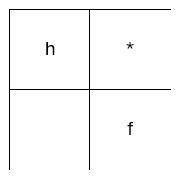
\includegraphics[width=0.4\textwidth]{images/biased_matching_pennies.png}
\captionof{figure}{Biased Matching Pennies}
\label{fig:biased_matching_pennies}
\end{minipage}

\subsection{Tree Maze Chase}
This scenario satisfies (\ref{eq:necessary_condition}). It essentially turns off the mixed strategy problem. We set up the game environment as follows.

\noindent
\begin{minipage}{\columnwidth}
\centering
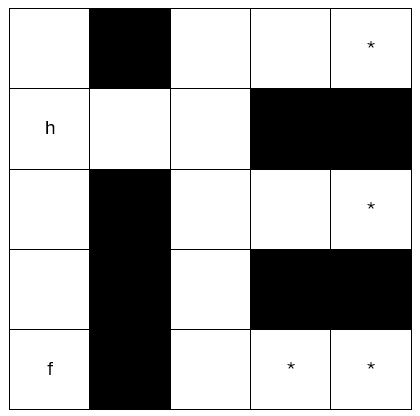
\includegraphics[width=0.8\textwidth]{images/tree_maze_chase.png}
\captionof{figure}{Tree Maze Chase}
\label{fig:tree_maze_chase}
\end{minipage}

\section{Results}
Figure \ref{fig:hopper_reward}, \ref{fig:frog_reward}, \ref{fig:snake_reward} shows the average test return for each type of agent after training in a randomly generated game environment. Figure \ref{fig:biased_matching_pennies_hopper_reward}, \ref{fig:biased_matching_pennies_frog_reward} demonstrates that in the carefully set up matching pennies scenario. The results show that the algorithms could not reach the optimal reward which can be computed using linear algebra (which is also another strong aspect of the game. we can analyse the game formally and see whether the agents reached optimality).

\noindent
\begin{minipage}{\columnwidth}
\centering
\includesvg[width=1\textwidth]{plots/rewards_global_hopper.svg}
\captionof{figure}{hopper rewards}
\label{fig:hopper_reward}
\end{minipage}

\noindent
\begin{minipage}{\columnwidth}
\centering
\includesvg[width=1\textwidth]{plots/rewards_global_frog.svg}
\captionof{figure}{frog rewards}
\label{fig:frog_reward}
\end{minipage}

\noindent
\begin{minipage}{\columnwidth}
\centering
\includesvg[width=1\textwidth]{plots/rewards_global_snake.svg}
\captionof{figure}{snake rewards}
\label{fig:snake_reward}
\end{minipage}

\noindent
\begin{minipage}{\columnwidth}
\centering
\includesvg[width=1\textwidth]{plots/rewards_scen_hopper.svg}
\captionof{figure}{biased matching pennies hopper rewards}
\label{fig:biased_matching_pennies_hopper_reward}
\end{minipage}

\noindent
\begin{minipage}{\columnwidth}
\centering
\includesvg[width=1\textwidth]{plots/rewards_scen_frog.svg}
\captionof{figure}{biased matching pennies frog rewards}
\label{fig:biased_matching_pennies_frog_reward}
\end{minipage}

\section{Discussion}

\section{Conclusion}

\section*{Funding}
This research was funded by the University of the West of England.

% Prints bibliography
\printbibliography

\end{multicols}
\end{document}